\documentclass[12pt,a4paper]{article}

\usepackage{amsmath,amssymb}
\usepackage{graphicx}
\usepackage{hyperref}
\usepackage{natbib}
\usepackage{geometry}
\usepackage{booktabs}
\usepackage{array}
\usepackage{xcolor}
\usepackage{setspace}
\usepackage{placeins}

\geometry{margin=1in}
\onehalfspacing

\hypersetup{
  colorlinks=true,
  linkcolor=black,
  citecolor=black,
  urlcolor=black
}

% ─────────────────────────────────────────────────────────────────────────────
\title{\textbf{Electroweak Symmetry Breaking and the Matter Sector}\\
\large Massive Timelike Worldlines, the Unbroken U(1), and the Composition of $\beta_m$\\
in the Informational Actualization Model}

\author{Heath W.\ Mahaffey\\
\small Independent Researcher, Entiat, WA 98822, USA\\
\small \texttt{hmahaffeyges@gmail.com}\\
\small \texttt{https://github.com/hmahaffeyges/IAM-Validation}}

\date{March 2026; revised October 2026}
% ─────────────────────────────────────────────────────────────────────────────

\begin{document}
\maketitle

\begin{abstract}
In the Informational Actualization Model (IAM) the matter sector is defined by
causal structure: degrees of freedom on timelike worldlines undergo gravitational
decoherence and produce informational entropy, while degrees of freedom on null
worldlines do not. This gives $\mu(a)<1$ for matter perturbations and $\Sigma(a)=1$
for light. Here we trace the particle-physics origin of that division. Electroweak
symmetry breaking at $T\approx100$ GeV ($t\approx10^{-11}$ s) gives the $W^\pm$,
$Z^0$ and the charged fermions their masses, placing them on timelike worldlines;
the unbroken U(1)$_{\rm em}$ keeps the photon exactly massless and on null
geodesics. Within IAM the transition is therefore the epoch at which a matter
sector capable of gravitational decoherence first exists, while the photon is
protected from it by an exact gauge symmetry. We separate what this establishes
from what it does not: photon masslessness guarantees that photons never enter
the matter sector, but $\Sigma=1$ remains a statement about how metric potentials
respond to matter and is tested by weak lensing. We also write the coupling
$\beta_m=\Omega_m/2$ as a sum of a baryonic part ($15.6\%$) and a dark-matter part
($84.4\%$), and we state the open question of whether the selection of the Higgs
vacuum is itself a decoherence event.
\end{abstract}

\noindent\textbf{Keywords:} electroweak symmetry breaking; Higgs mechanism; virial
theorem; gravitational decoherence; CP violation; baryon asymmetry; $\mu$--$\Sigma$
framework; Informational Actualization Model

% ─────────────────────────────────────────────────────────────────────────────
\section{Introduction}
\label{sec:intro}

IAM identifies an informational contribution to horizon entropy produced by
gravitational decoherence during structure formation \citep{mahaffey2026}. The
contribution enters the matter-sector perturbation equations through an enhanced
Hubble friction and leaves photon propagation unchanged, so that
$\mu(a)=E^2_{\Lambda\rm CDM}(a)/E^2_{\rm IAM}(a)<1$ and $\Sigma(a)=1$. The division
rests on a single criterion: a degree of freedom decoheres gravitationally only if
it accumulates proper time, $\Delta\tau>0$.

That criterion has a particle-physics history. Above the electroweak scale the
Standard Model gauge bosons and fermions are massless, and their excitations
propagate on null geodesics. The Higgs mechanism gives them mass. This paper sets
out what the electroweak transition contributes to the IAM picture, what it does
not, and which statements are testable.

% ─────────────────────────────────────────────────────────────────────────────
\section{The virial theorem and the interactions}
\label{sec:virial}

For a bound system with potential energy homogeneous of degree $k$ in the
coordinates, $V(\lambda r)=\lambda^k V(r)$, the time-averaged virial theorem gives
\begin{equation}
  2\langle K\rangle = k\,\langle V\rangle .
  \label{eq:virial}
\end{equation}
For the $1/r$ potentials of Newtonian gravity and electrostatics, $k=-1$ and
$2\langle K\rangle+\langle V\rangle=0$ \citep{clausius1870}. This relation holds for
atoms and molecules (to the precision of their computed ground states), for stars
and galaxy clusters, and it is the basis of the IAM coupling $\beta_m=\Omega_m/2$
\citep{mahaffey2026_thermo_virial}. In IAM the kinetic half $\langle K\rangle$ is
identified with the heat released irreversibly at virialisation, the Landauer cost
of the quantum-to-classical transition.

The strong interaction is different. The static quark potential is well described
by the Cornell form $V(r)=-\tfrac{4}{3}\alpha_s/r+\sigma r$, with string tension
$\sigma\approx0.18$ GeV$^2$: Coulomb-like ($k=-1$) at short distance and linear
($k=+1$) at the confinement scale, where Eq.~(\ref{eq:virial}) gives
$2\langle K\rangle=+\langle V_{\rm lin}\rangle$. Hadrons are virialised bound states,
but of their own potential, not of the $1/r$ form. The weak interaction forms no
bound states at all: its range, $\sim\hbar/(M_W c)\approx2.5\times10^{-18}$ m, is
set by the $W$ mass, and its role is to change flavour.

% ─────────────────────────────────────────────────────────────────────────────
\section{The weak interaction: flavour change and the discrete symmetries}
\label{sec:weak}

The weak interaction, mediated by $W^\pm$ ($80.4$ GeV) and $Z^0$ ($91.2$ GeV), is
the only interaction that changes quark and lepton flavour. It drives beta decay
and the first step of the proton--proton chain. It violates parity maximally
\citep{wu1957} and violates CP through the phase of the CKM matrix
\citep{cronin1964,ckm1973}; by the CPT theorem it therefore violates time-reversal
symmetry at the level of fundamental interactions.

Two points matter here.
\begin{enumerate}
  \item CP violation is one of the three Sakharov conditions for generating a
  baryon asymmetry \citep{sakharov1967}. The measured asymmetry,
  $\eta=(6.12\pm0.04)\times10^{-10}$ \citep{planck2020}, fixes $\Omega_b$. The CKM
  phase alone is too small to produce it, and in the Standard Model the electroweak
  transition is a smooth crossover rather than the first-order transition that
  electroweak baryogenesis requires; the mechanism that set $\eta$ is unknown.
  \item The thermodynamic arrow of time does not require CP violation. Entropy
  production, decoherence and Landauer's bound hold for any interaction. What the
  electroweak transition adds is not irreversibility but massive particles.
\end{enumerate}

% ─────────────────────────────────────────────────────────────────────────────
\section{Electroweak symmetry breaking and the IAM sectors}
\label{sec:ewsb}

\subsection{Before the transition}
Above $T\approx160$ GeV the Higgs expectation value vanishes in the Standard Model.
The $W$, $Z$ and the fermions have no rest mass (they carry thermal masses from the
plasma, which do not change their light-like dispersion at high momentum). In the
IAM criterion they do not accumulate proper time and do not decohere
gravitationally. In any case the activation function is negligible at these epochs:
$E(a)=\exp(1-1/a)$ is $\exp(-10^{15})$ at $T\sim100$ GeV and only
$E(z=10)=4.5\times10^{-5}$ at the onset of structure.

\subsection{The transition}
As the universe cools through the electroweak scale the Higgs field acquires its
vacuum expectation value $v=246$ GeV. The $W^\pm$ and $Z^0$ acquire mass, the
charged fermions acquire masses $m_f=y_f v/\sqrt2$, and their excitations move on
timelike worldlines with $\Delta\tau>0$. In IAM language the matter sector exists
from this epoch onward. (Dark matter, whose particle nature is unknown, joins the
matter sector by the same criterion if it is massive.)

\subsection{The unbroken U(1) and the photon sector}
The electromagnetic U(1) survives the transition unbroken, so the photon remains
exactly massless; the experimental bound is $m_\gamma<10^{-18}$ eV \citep{pdg2022}.
Photons therefore stay on null geodesics, accumulate no proper time, and by the IAM
criterion never produce informational entropy. This makes the photon exemption a
consequence of an established symmetry rather than an extra assumption.

It does not by itself establish $\Sigma=1$. The quantity $\Sigma$ describes how the
lensing potential $\Phi+\Psi$ responds to the matter distribution. In IAM
$\Sigma=1$ follows from $\delta\phi=0$ and the absence of anisotropic stress in the
informational sector \citep{mahaffey2026}. Euclid weak lensing, with projected
$\sigma(\Sigma_0)\approx0.02$ \citep{euclid2020}, tests it directly.

% ─────────────────────────────────────────────────────────────────────────────
\section{The sequence of bound structures}
\label{sec:sequence}

Figure~\ref{fig:timeline} and Table~\ref{tab:sequence} place the transition in the
standard thermal history. Times and energies are standard cosmology and the
Standard Model \citep{pdg2022}; the grand-unification entry is a hypothesis.

\begin{figure}[!htbp]
  \centering
  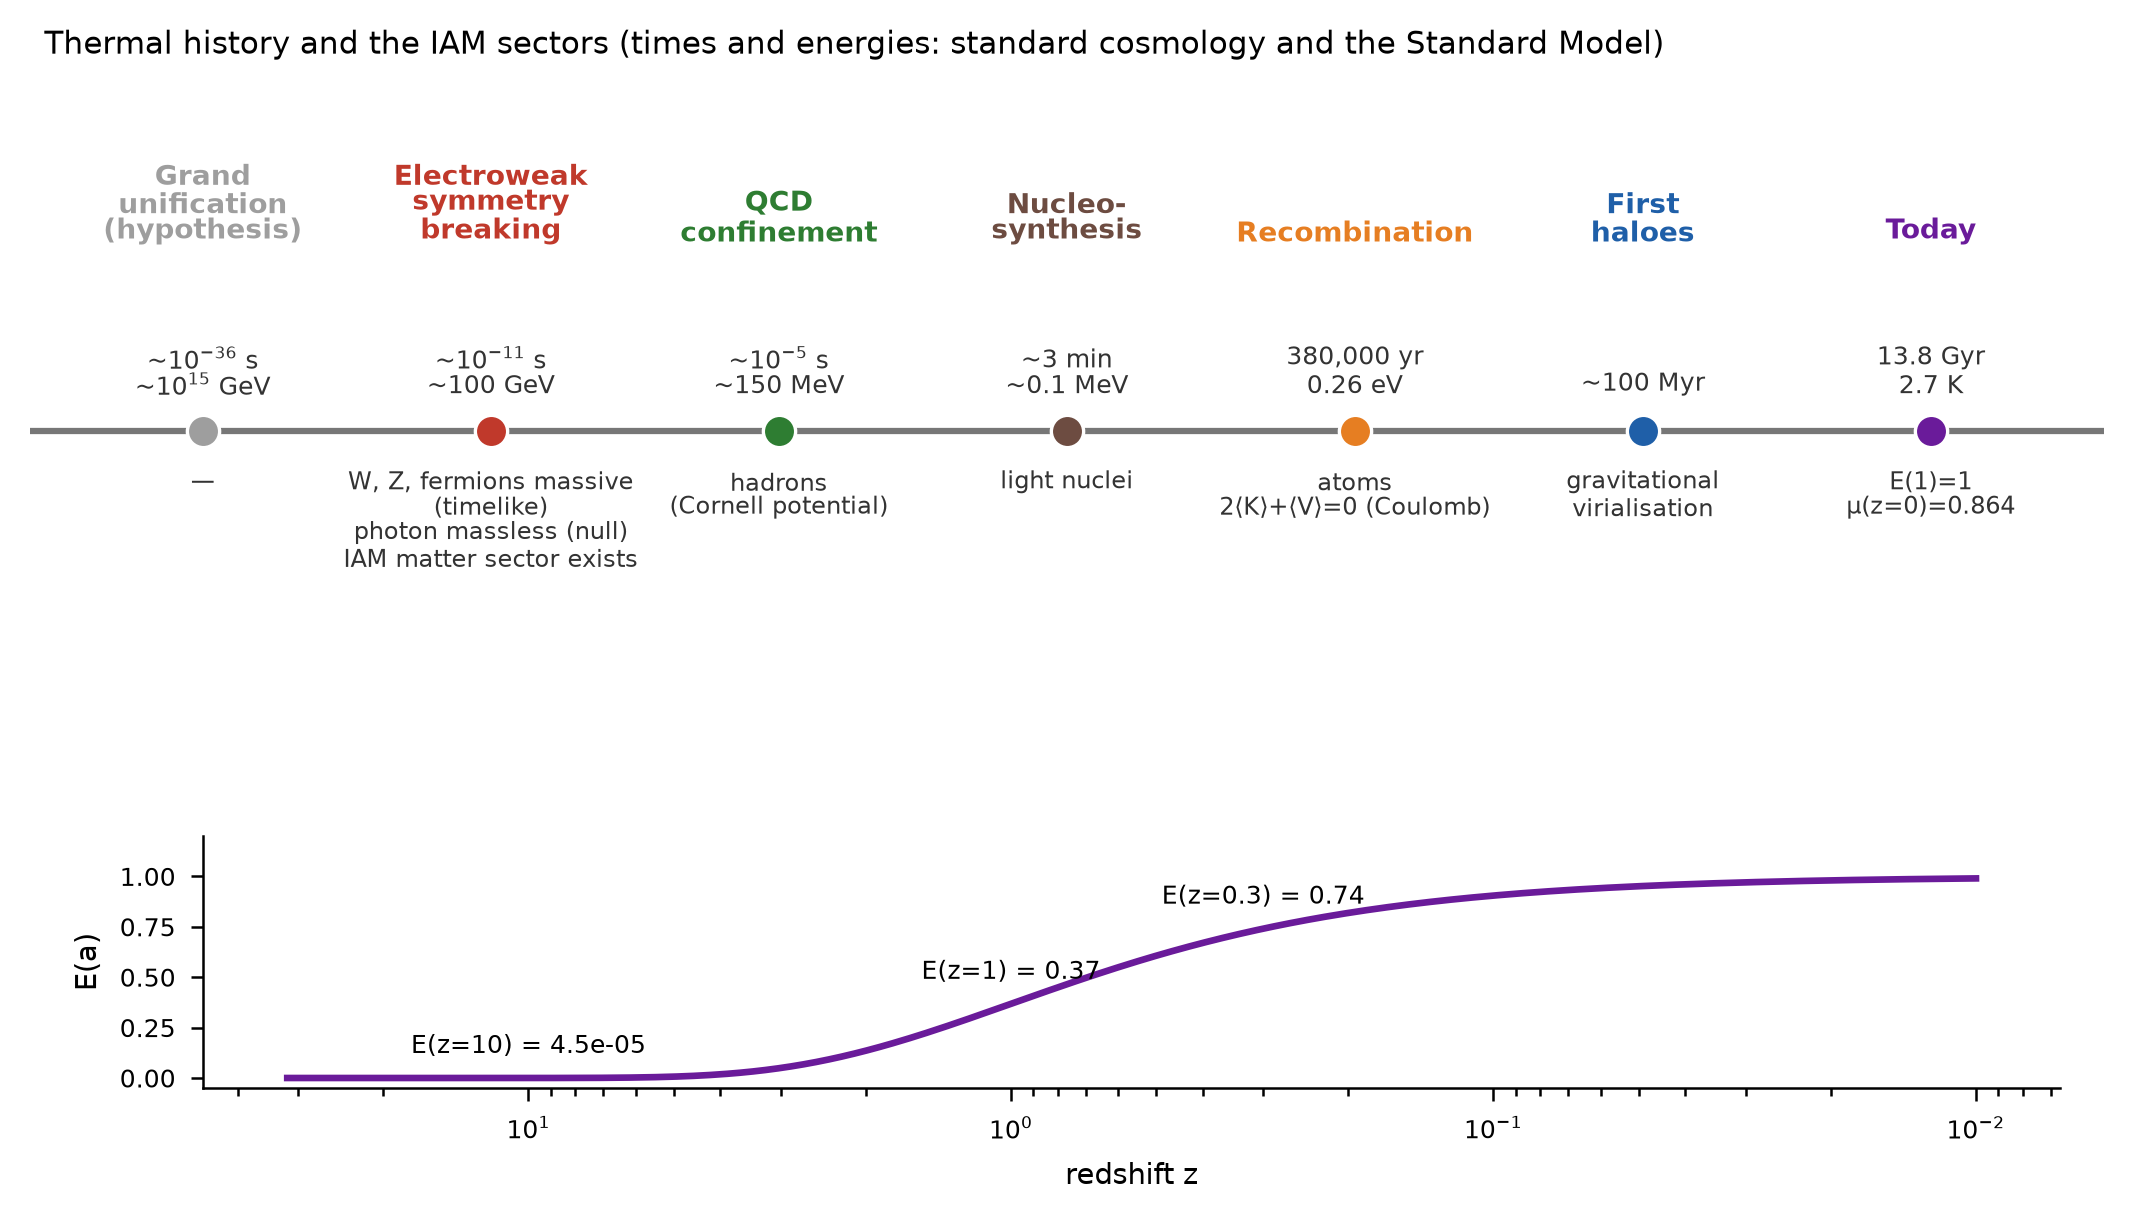
\includegraphics[width=0.97\textwidth]{iam_electroweak_timeline.png}
  \caption{Thermal history and the IAM sectors. Electroweak symmetry breaking gives
  the massive particles of the matter sector; the photon remains massless under the
  unbroken U(1). Bound structures then form at increasing scales (hadrons, atoms,
  haloes). The activation function $E(a)=\exp(1-1/a)$ (purple) is negligible until
  the late universe, where it reaches $E(z=1)=0.37$ and $E(z=0)=1$.}
  \label{fig:timeline}
\end{figure}

\begin{table}[!htbp]
\centering
\caption{Thermal history and the formation of bound structures.}
\label{tab:sequence}
\begin{tabular}{p{2.2cm} p{2.0cm} p{3.4cm} p{5.6cm}}
\toprule
Time & Temperature & Event & Consequence \\
\midrule
$\sim10^{-36}$ s & $\sim10^{15}$ GeV & Grand unification (hypothesis) & --- \\
$\sim10^{-11}$ s & $\sim100$ GeV & Electroweak symmetry breaking & $W$, $Z$, fermions massive (timelike); photon massless (null); IAM matter sector exists \\
$\sim10^{-5}$ s & $\sim150$ MeV & QCD confinement & Hadrons: bound states of the Cornell potential \\
$\sim3$ min & $\sim0.1$ MeV & Nucleosynthesis & Light nuclei; $\Omega_b$ already fixed by $\eta$ \\
$380{,}000$ yr & $0.26$ eV & Recombination & Atoms: $2\langle K\rangle+\langle V\rangle=0$ (Coulomb) \\
$\sim100$ Myr & --- & First haloes & Gravitational virialisation; $E(z\approx30)\approx10^{-13}$ \\
$\sim13.8$ Gyr & 2.7 K & Today & $E(1)=1$; $\mu(z=0)=0.864$ \\
\bottomrule
\end{tabular}
\end{table}

% ─────────────────────────────────────────────────────────────────────────────
\section{The composition of $\beta_m$}
\label{sec:beta}

The coupling $\beta_m=\Omega_m/2$ follows from the virial partition of gravitational
energy \citep{mahaffey2026,mahaffey2026_thermo_virial}. With Planck 2018 values
\citep{planck2020}, $\Omega_m=0.3153$ and $\Omega_b=0.0493$:
\begin{equation}
  \beta_m = \frac{\Omega_b}{2} + \frac{\Omega_{dm}}{2}
          = 0.0247 + 0.1332 = 0.15765 .
  \label{eq:beta}
\end{equation}
The baryonic part ($15.6\%$) is fixed by the baryon asymmetry, whose origin
requires CP violation and lies beyond the Standard Model (Sec.~\ref{sec:weak}).
The dark-matter part ($84.4\%$) is fixed by the dark-matter density. Both are
measured inputs; $\beta_m$ introduces no parameter beyond them. A change in the
measured $\Omega_m$ shifts $\beta_m$ in proportion, $\beta_m/\Omega_m=1/2$, which is
itself testable by refitting with different $\Omega_m$ priors \citep{mahaffey2026}.

% ─────────────────────────────────────────────────────────────────────────────
\section{Open question: is vacuum selection a decoherence event?}
\label{sec:open}

The Higgs field settles into one point of a degenerate vacuum manifold. In a
quantum treatment the early field is in a superposition over that manifold, and the
emergence of a definite classical vacuum requires decoherence through coupling to
the other fields of the plasma. If so, the selection of the vacuum is itself an
irreversible quantum-to-classical transition, carrying a Landauer cost at the
temperature of the transition. IAM does not yet treat this event, and nothing in the
cosmological predictions depends on it. We state it as an open problem: whether the
electroweak vacuum selection can be described within the decoherence framework of
Ref.~\citep{mahaffey2026}, and whether it leaves any observable trace.

% ─────────────────────────────────────────────────────────────────────────────
\section{Tests}
\label{sec:tests}

\begin{enumerate}
  \item $\Sigma_0=0$: Euclid weak lensing at $\sigma(\Sigma_0)\approx0.02$. A
  significant nonzero $\Sigma_0$ falsifies the IAM photon exemption.
  \item $\mu_0=-0.136$ ($\mu(z=0)=0.864$): Euclid clustering, forecast detection
  $3.4\sigma$ (optimistic) and $5.4\sigma$ with DESI Year 5 \citep{mahaffey2026}.
  \item $\beta_m/\Omega_m=1/2$: holds for any revision of $\Omega_m$.
\end{enumerate}

% ─────────────────────────────────────────────────────────────────────────────
\section{Conclusions}

Electroweak symmetry breaking gives mass to the $W$, $Z$ and the charged fermions
and leaves the photon massless under the unbroken U(1). Within IAM this is the epoch
from which a matter sector able to decohere gravitationally exists, and the photon's
exact masslessness keeps it permanently outside that sector. The cosmological
signature, $\mu<1$ with $\Sigma=1$, is set much later by structure formation and is
tested by Euclid. The coupling $\beta_m=0.15765$ is the sum of a baryonic part fixed
by the unexplained baryon asymmetry and a dark-matter part, with no free parameter.
Whether the selection of the electroweak vacuum is itself a decoherence event is
left open.

% ─────────────────────────────────────────────────────────────────────────────
\section*{Data Availability}
Analysis scripts are available at \url{https://github.com/hmahaffeyges/IAM-Validation}.

\bibliographystyle{plainnat}
\begin{thebibliography}{99}
\bibitem[Clausius(1870)]{clausius1870} Clausius, R.\ 1870, Phil.\ Mag., 40, 122
\bibitem[Cronin \& Fitch(1964)]{cronin1964} Cronin, J.\ W.\ \& Fitch, V.\ L.\ 1964, Phys.\ Rev.\ Lett., 13, 138
\bibitem[Cabibbo(1963); Kobayashi \& Maskawa(1973)]{ckm1973} Cabibbo, N.\ 1963, Phys.\ Rev.\ Lett., 10, 531; Kobayashi, M.\ \& Maskawa, T.\ 1973, Prog.\ Theor.\ Phys., 49, 652
\bibitem[Euclid Collaboration et al.(2020)]{euclid2020} Euclid Collaboration, Blanchard, A., et al.\ 2020, A\&A, 642, A191
\bibitem[Mahaffey(2026a)]{mahaffey2026} Mahaffey, H.\ W.\ 2026a, Horizon Thermodynamics and Gravitational Decoherence as the Origin of $\mu<1$, $\Sigma=1$, preprint
\bibitem[Mahaffey(2026b)]{mahaffey2026_thermo_virial} Mahaffey, H.\ W.\ 2026b, The Thermodynamic Identity Governing the Virial Theorem, preprint
\bibitem[Particle Data Group(2022)]{pdg2022} Particle Data Group, Workman, R.\ L., et al.\ 2022, Prog.\ Theor.\ Exp.\ Phys., 2022, 083C01
\bibitem[Planck Collaboration(2020)]{planck2020} Planck Collaboration, Aghanim, N., et al.\ 2020, A\&A, 641, A6
\bibitem[Sakharov(1967)]{sakharov1967} Sakharov, A.\ D.\ 1967, JETP Lett., 5, 24
\bibitem[Wu et al.(1957)]{wu1957} Wu, C.\ S., et al.\ 1957, Phys.\ Rev., 105, 1413
\end{thebibliography}
\end{document}
